\subsection{Shared discrepancy and matched temporal smoothness}

    The preceding forecasts systematically underpredict later observations.
    We investigate two hypotheses while keeping the logistic median and its
    parameter priors fixed: a departure common to all trials, and smoother
    temporal evolution of that departure. This is an exploratory comparison
    prompted by the observed residuals. It does not supply an untouched test
    set or establish a physical cause. Allowing model discrepancy also changes
    what can be learned about the mechanistic parameters
    \citep{brynjarsdottir2014discrepancy}.
    Mean-based scores below use the saved finite posterior subsets; their
    full-posterior moment limitation is established in
    Section~\ref{sec:predictive-moments}.

    Let \(A_{ik}=a^2 c(|s_i-s_k|)\). The independent model retains one
    discrepancy process per trial; the shared model instead uses
    \[
        \log Y_i^{[j]}=\log m_\theta(s_i)+D(s_i)+\varepsilon_i^{[j]},
        \qquad \varepsilon_i^{[j]}\overset{\mathrm{iid}}{\sim}\mathcal N(0,b^2).
    \]
    Logarithms use the response reference unit defined in the preceding
    section. Shared discrepancy can represent a common departure from the
    logistic median. It is a different assumption about trial dependence,
    rather than an additional source of independent flask variability.
    In time-major ordering, the two covariance models are
    \[
        C_{\rm independent}=A\otimes I_J+b^2 I_{nJ},\qquad
        C_{\rm shared}=A\otimes\boldsymbol 1_J\boldsymbol 1_J^\top+b^2 I_{nJ},
        \qquad J=3.
    \]
    No model in this comparison contains both shared and trial-specific
    correlated deviations. Nor do the shared models contain trial random
    intercepts. Their measurement errors absorb the remaining trial contrasts;
    these modeling restrictions require experimental justification.

    A two-by-two comparison crosses these dependence assumptions with
    \[
        c_{\rm OU}(d)=e^{-\lambda d},\qquad
        c_{3/2}(d)=(1+\kappa d)e^{-\kappa d},\qquad
        \kappa=\xi\lambda,
    \]
    where \((1+\xi)e^{-\xi}=e^{-1}\), so \(\xi\simeq2.14619\).
    Both kernels therefore have stationary variance \(a^2\) and e-fold
    correlation time \(12/\lambda\) in original time units. Using the same
    prior for \(\lambda\) thus matches this time-scale summary rather than
    silently changing it when smoothness changes. The Mat\'ern process has
    an exact two-state linear SDE representation
    \citep[Example 12.7]{sarkka2019applied}:
    \[
        d\begin{pmatrix}D\\V\end{pmatrix}
        =\begin{pmatrix}0&1\\-\kappa^2&-2\kappa\end{pmatrix}
         \begin{pmatrix}D\\V\end{pmatrix}ds
        +\begin{pmatrix}0\\2a\kappa^{3/2}\end{pmatrix}dW,
        \qquad
        P_\infty=\operatorname{diag}(a^2,a^2\kappa^2).
    \]
    This supplies a velocity state for conditional forecasts. Neither kernel
    introduces a permanent departure from the logistic asymptote: both have
    stationary zero-mean discrepancies.

\subsection{Exact inference and forecast scoring}

    The shared likelihood is evaluated through an orthogonal decomposition
    across trials. The transformed mean \(\sqrt J\,\bar r\) has covariance
    \(JA+b^2I_n\), and the \(J-1\) orthogonal contrasts have covariance
    \(b^2I_n\). Gaussian conditioning of the common discrepancy uses the
    mean residual with covariance \(A+(b^2/J)I_n\). The joint predictive
    density retains the shared covariance between future trials; multiplying
    their marginal densities would give an incorrect joint score. Dense
    Gaussian likelihood and conditioning calculations independently check
    these reductions. Stationary Lyapunov and matrix-exponential identities
    check the two kernels against their SDE representations.

    All four models retain the six-coordinate priors and half/double noise
    sensitivity analysis from the preceding section, with four chains and
    the same computational acceptance criteria. Earlier validated independent
    OU samples are reused after checking inference-source and data hashes;
    recomputed forecasts agree with their saved values. Three new model
    alternatives are fitted at cutoffs 108, 120, 132, and 168 under all three
    priors. All four models are also fitted at cutoffs 144 and 156 under the
    reference prior. This gives 56 posterior cases including 12 reused cases.

    The original multi-time holdouts retain their 36 entries and overlapping
    targets. An additional one-step comparison trains through
    \(108,120,132,144,156\) and predicts only the immediately following
    time. Its 15 scalar responses each appear once, with parameters refitted
    using the available past. This removes repeated scoring of the same
    response from that summary, but does not make successive responses or
    the three trial trajectories independent experiments.

    Alongside coverage, RMSE, signed bias, and marginal and joint negative
    log predictive density, we report the central 90 percent interval score:
    \[
        S_{0.1}(l,u;y)=(u-l)
        +20(l-y)\boldsymbol 1_{\{y<l\}}
        +20(y-u)\boldsymbol 1_{\{y>u\}}.
    \]
    Smaller scores are preferable. The width term penalizes broad intervals,
    so nominal coverage alone cannot determine which model forecasts better.
    Joint density scores account for within-forecast dependence, but their
    overlapping multi-time summaries remain descriptive.

% Generated by scripts/build_structural_tables.py; do not edit manually.
\begin{table}[htbp]
\centering
\caption{Multi-time holdouts: 36 overlapping forecast entries per model. Reference prior; nominal coverage 0.90. IS is the interval score; NLL columns are marginal and joint per-entry negative log predictive density.}
\label{tab:structural-rollout}
\begingroup\small\setlength{\tabcolsep}{4pt}
\begin{tabular}{lrrrrr}
\toprule
Model & Coverage & Width & IS & Marg. NLL & Joint NLL \\
\midrule
Independent OU & 0.8056 & 5.857 & 10.164 & 2.404 & 2.196 \\
Shared OU & 0.9722 & 9.138 & 9.371 & 2.273 & 2.280 \\
Independent Mat\'ern & 0.8056 & 5.833 & 10.211 & 2.412 & 2.197 \\
Shared Mat\'ern & 0.9444 & 9.017 & 9.667 & 2.309 & 2.301 \\
\bottomrule
\end{tabular}
\endgroup
\end{table}
\begin{table}[htbp]
\centering
\caption{One-step forecasts: 15 distinct scalar targets per model. Reference prior; nominal coverage 0.90. IS is the interval score; NLL columns are marginal and joint per-entry negative log predictive density.}
\label{tab:structural-one-step}
\begingroup\small\setlength{\tabcolsep}{4pt}
\begin{tabular}{lrrrrr}
\toprule
Model & Coverage & Width & IS & Marg. NLL & Joint NLL \\
\midrule
Independent OU & 0.8667 & 5.655 & 8.224 & 2.099 & 2.061 \\
Shared OU & 0.9333 & 7.145 & 7.489 & 1.991 & 2.118 \\
Independent Mat\'ern & 0.8667 & 5.639 & 8.217 & 2.099 & 2.060 \\
Shared Mat\'ern & 0.9333 & 7.128 & 7.847 & 2.038 & 2.136 \\
\bottomrule
\end{tabular}
\endgroup
\end{table}
\begin{table}[htbp]
\centering
\caption{Full-data logistic capacity posterior under the reference prior. These are parameter credible intervals, not observation predictive intervals.}
\label{tab:structural-capacity}
\begingroup\small\setlength{\tabcolsep}{4pt}
\begin{tabular}{lrrr}
\toprule
Model & Median & 5th percentile & 95th percentile \\
\midrule
Independent OU & 48.012 & 47.177 & 49.050 \\
Shared OU & 48.337 & 45.555 & 52.107 \\
Independent Mat\'ern & 48.010 & 47.217 & 49.003 \\
Shared Mat\'ern & 48.144 & 46.369 & 50.928 \\
\bottomrule
\end{tabular}
\endgroup
\end{table}
\begin{table}[htbp]
\centering
\caption{Multi-time forecast sensitivity across half, reference, and double noise-prior medians. Ranges summarize three fixed choices, not optimized hyperparameters.}
\label{tab:structural-sensitivity}
\begingroup\small\setlength{\tabcolsep}{4pt}
\begin{tabular}{lrrrr}
\toprule
Model & Min. coverage & Max. coverage & Min. IS & Max. IS \\
\midrule
Independent OU & 0.7778 & 0.8333 & 9.921 & 10.359 \\
Shared OU & 0.9444 & 1.0000 & 9.052 & 10.068 \\
Independent Mat\'ern & 0.7500 & 0.8333 & 9.946 & 10.445 \\
Shared Mat\'ern & 0.9444 & 0.9722 & 9.069 & 10.088 \\
\bottomrule
\end{tabular}
\endgroup
\end{table}


\subsection{Results and remaining scientific limits}

    For multi-time holdouts, reference shared OU coverage is
    0.9722, compared with 0.8056 for independent
    OU deviations. Mean width changes from 5.857 to
    9.138; interval score changes from
    10.164 to 9.371.
    Mean observed-minus-predicted bias remains 1.373
    for shared OU, versus 1.648 for independent OU.
    Their RMSE values are 2.195 and 2.411, respectively.
    Improved coverage therefore must be interpreted together with interval
    width, scoring rules, and residual bias, rather than as a correction of
    the logistic growth law.

    On the distinct one-step targets, shared and independent OU coverage are
    0.9333 and 0.8667; their interval scores are
    7.489 and 8.224.
    Marginal NLL values are 1.991 and
    2.099, and joint per-entry NLL values are
    2.118 and
    2.061.
    The joint score evaluates the three simultaneous trial responses together,
    retaining both latent dependence and common parameter uncertainty.
    Here the shared OU model improves marginal NLL and interval score,
    whereas independent OU has the better joint predictive density score
    under both forecast summaries. This disagreement matters: the marginal
    improvement does not validate the stronger shared-dependence assumption.

    Smoother independent Mat\'ern discrepancies have multi-time coverage
    0.8056 and mean bias
    1.653; shared Mat\'ern
    discrepancies have coverage 0.9444
    and bias 1.362.
    Table~\ref{tab:structural-one-step} reports their distinct-target scores.
    This fixed comparison does not establish that temporal smoothness resolves
    the late systematic departure. No candidate is promoted to a mechanistic
    reference on these retrospective data.

    All 56 posterior cases meet the computational thresholds: largest
    $\widehat R=1.0070$, minimum bulk ESS
    641, and minimum tail ESS
    444. New cases retain between
    36000 and
    108000 draws per chain
    after 6000 warmup iterations. A conditional-mixture integration check at
    cutoff 132 uses 6000, 12000, and 24000 posterior draws for the three new
    alternatives. Its largest endpoint shift from the 6000-draw result is
    0.044 response units.
    This is a finite numerical sensitivity check, not proof of predictive calibration.

    Shared discrepancy permits a wider range of population capacities
    (Table~\ref{tab:structural-capacity}). Broader capacity uncertainty is
    consistent with confounding between a common trajectory departure and
    the logistic median. The exploratory noise priors do not identify a
    unique physical decomposition. Noise-prior sensitivity, limited trial
    replication, and the unconfirmed physical units remain substantive
    limitations. The next validation step is to freeze the model comparison,
    confirm measurement units and experimental dependence, and assess
    additional independently collected trajectories with forecasts specified
    before inspecting their outcomes. REV-07 remains scientifically open.

\begin{figure}[htbp]
    \centering
    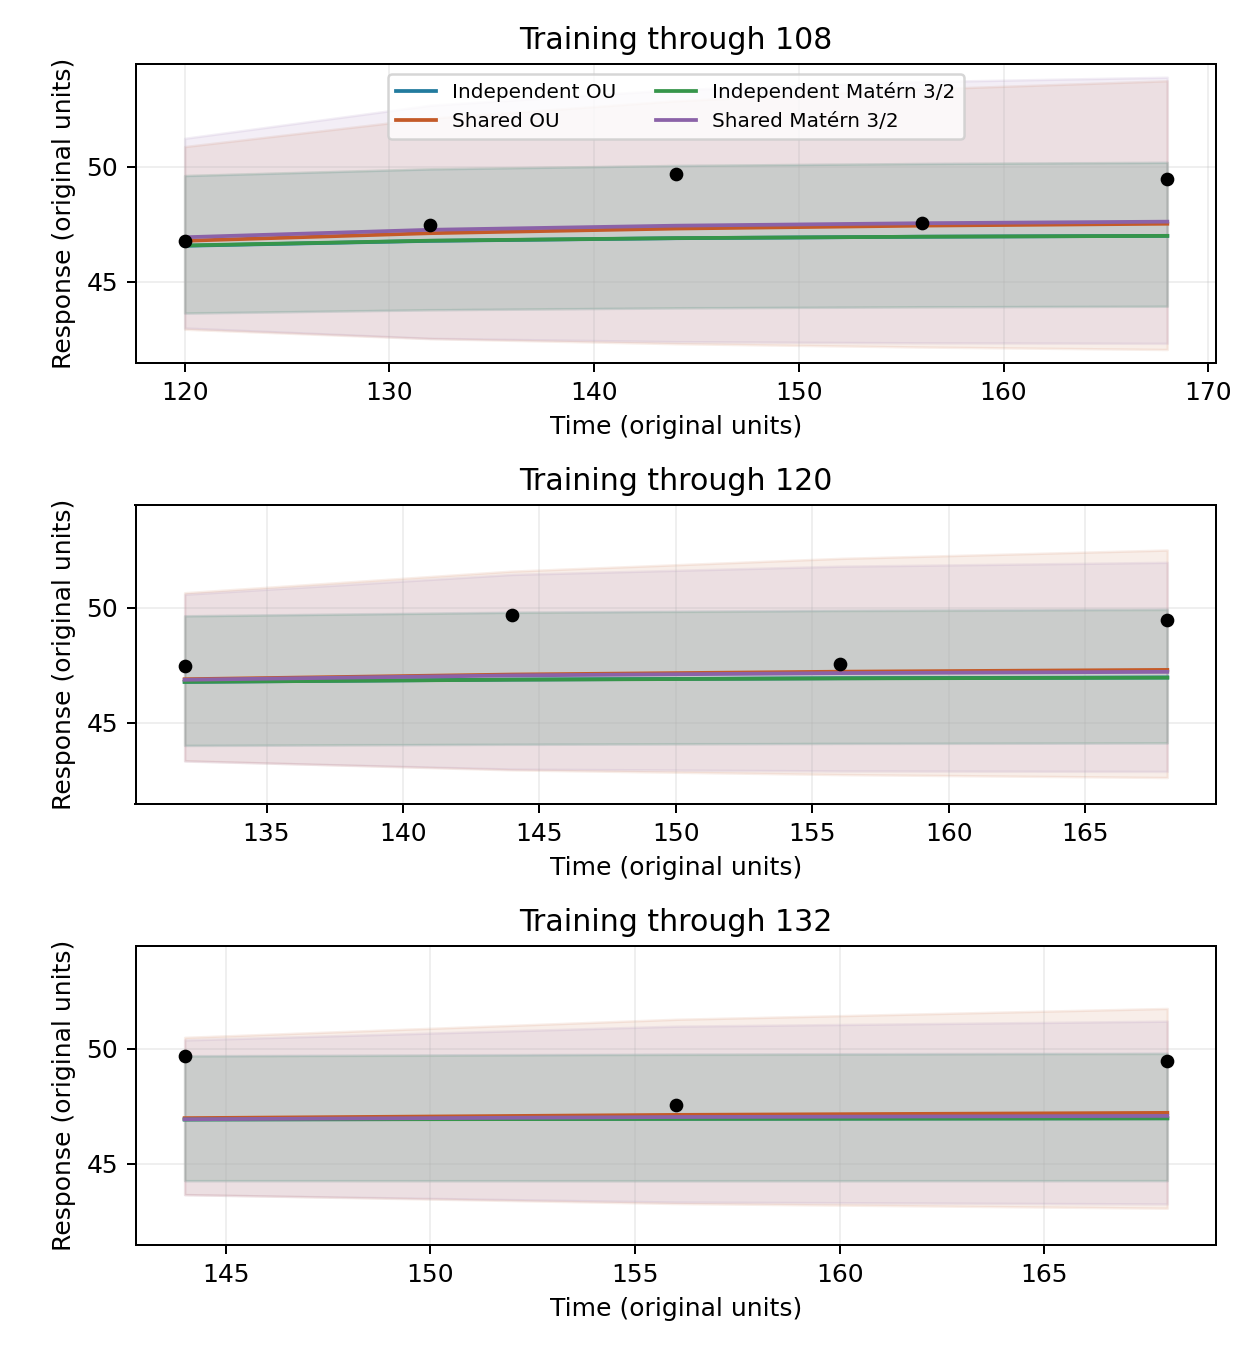
\includegraphics[width=\textwidth]{../results/structural/forecast_comparison.png}
    \caption{Matched structural alternatives, reference priors: trial 1
    predictive means and central 90 percent observation intervals. Black
    points are held-out responses. All reported scores use all three trials.}
    \label{fig:structural-forecast}
\end{figure}
\begin{figure}[htbp]
    \centering
    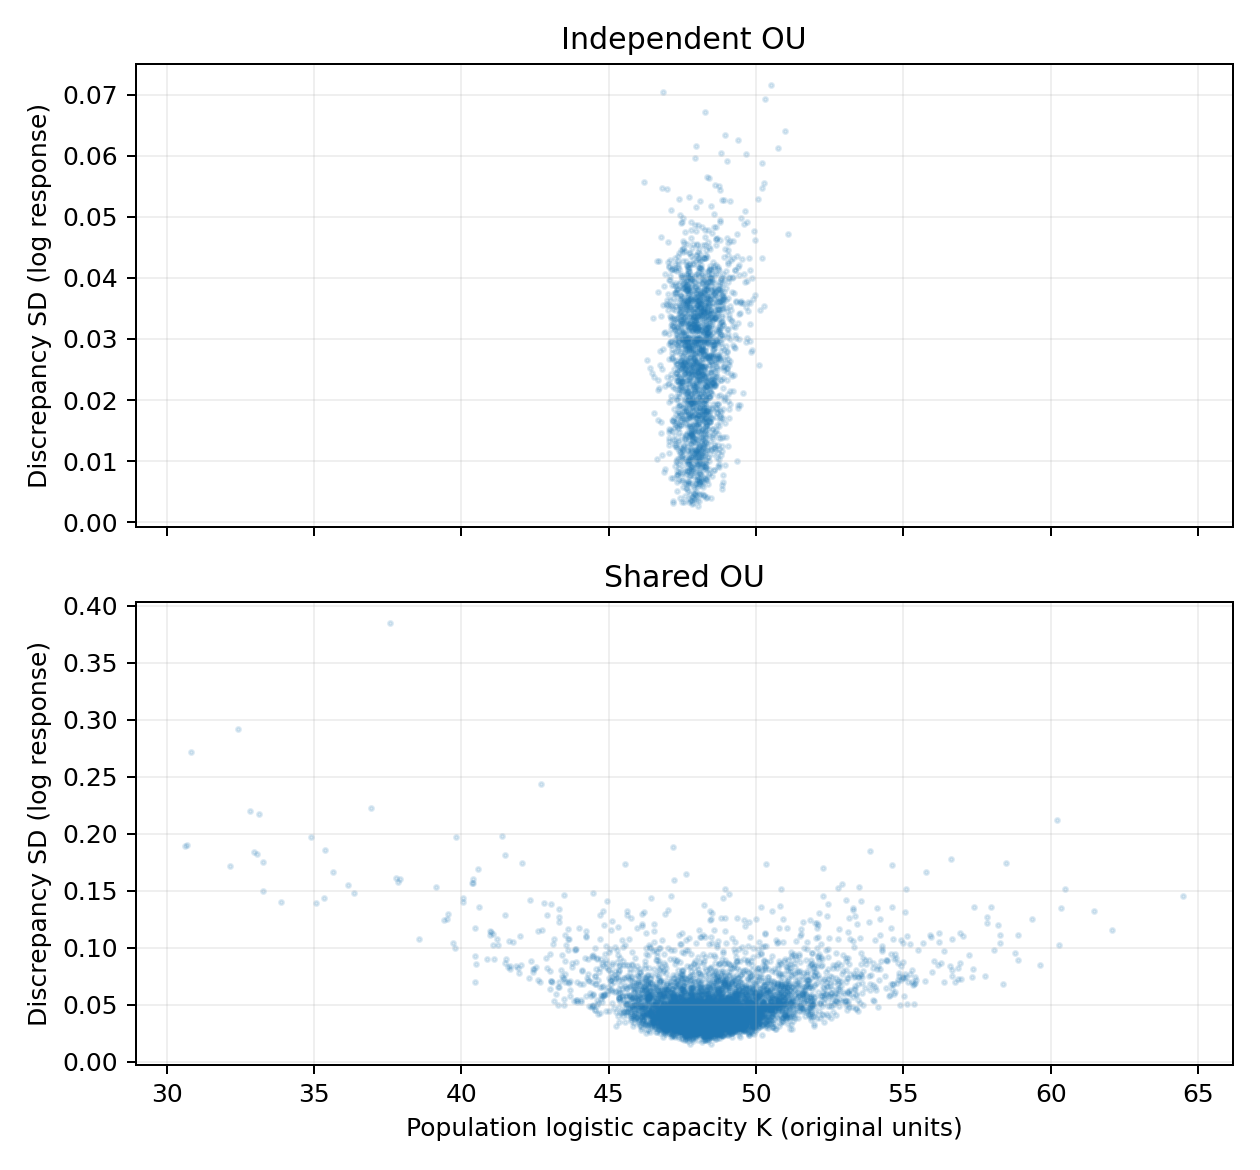
\includegraphics[width=0.9\textwidth]{../results/structural/capacity_discrepancy.png}
    \caption{Full-data reference posterior samples for capacity and discrepancy
    amplitude under independent and shared OU assumptions. The shared model
    allows greater uncertainty in the population capacity.}
    \label{fig:structural-capacity}
\end{figure}

